\section{Introduction}
Un \textit{terminal passif\footnote{Un dispositif d’affichages et de saise simples qui ne réalisent pas de traitement important et dépend d’une unité centrale.}}, était au début, un périphérique physique connecté à une unité centrale appelé un \textit{mainframe\footnote{Un ordinateur qui sert d'unité centrale pour des réseaux de terminaux.}}.
Ce terminal était seulement un dispositif d'entrées/sorties et ne pouvait pas traiter les données seuls sans le mainframe. C'était le mainframe qui traitait les données et renvoyait le résultat au terminal passif pour affichage.

\begin{figure}[h]
    \centering
    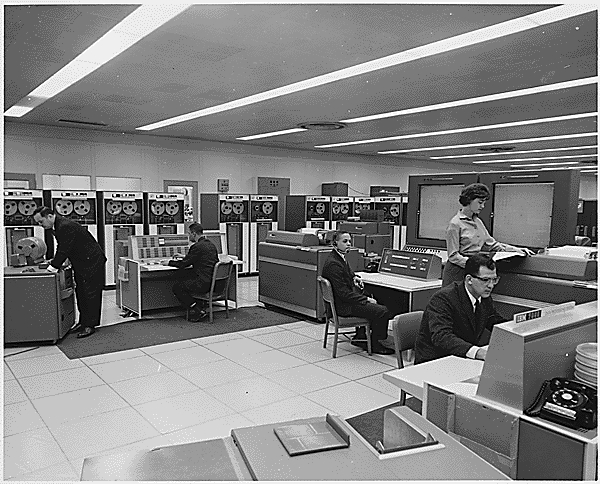
\includegraphics[width=0.8\linewidth]{images/mainframe.jpeg}
    \caption{Ordinateur de la NASA en 1962.}
\end{figure}

Aujourd'hui, avec l'avènement des ordinateurs personnels, ces derniers sont capables de traiter les données de manière autonome sans nécessiter un mainframe. Les terminaux ne sont plus nécessairement physiques aujourd'hui, mais peuvent être émulés de manière virtuelle par le système d'exploitation.

Pour pouvoir intéragir avec le système d'exploitation en utilisant un terminale virtuelle, il faut passer par une \textbf{console virtuelle}. Le répertoire spécial qui régroupe tout les périphériques utiliser par la machine est \textbf{/dev}. Dans ce répertoire, il y'a au total 64 fichiers spéciaux nommé \textbf{tty} (pour TeleTYpewriter).
Chaque fichier \textbf{tty} représente une console virtuelle qui peut être utilisé en tapant les touches \textit{CTRL+ALT+F[1 à 6]}.

Une console virtuelle permet d'établir une communication entre l'utilisateur et le noyau. Quand l'utilisateur entre une commande, il est interprété par le shell. L'utilisation d'une console virtuelle est possible uniquement dans un environnement non graphique. 
Tandis que dans un environnement graphique, il existe différent \textbf{émulateur de terminal} qui permettent de utiliser un terminal graphique, il existe entre autre un émulateur de terminal comme \textbf{xterm}.

Le point commun entre ces 2 types de terminaux virtuelles c’est qu’ils utilisent un \textbf{pseudo-terminal}. Un pseudo-terminal est un périphérique virtuel qui permet d’établir une communication bidirectionnelle et asynchrone entre 2 ou plusieurs procesuss. Un processus (esclave) fournis une interface qui est comme un termnial classique et l'autre processus (maître) va contrôler ce terminal.
